
The results of performance metrics  
measurements (\ref{sec:performance-metrics}) of Zigbee and Thread
networks are presented and discussed throughout this chapter. Tests
were executed on networks consisting of 7 devices
and followed the procedures described in chapter \ref{chap:research_methodology}.

\section{Latency}

\subsection{Latency in Thread networks}

Thread latency measurement results are presented in the table 
\ref{table:thread_latency}. A graphical representation of latency dependency on the
number of hops is shown in Fig. \ref{fig:thread_latency_all}, whereas Fig. \ref{fig:thread_latency_length} shown the latency in
the function of packet length.

\begin{figure}[H]
    \centering
    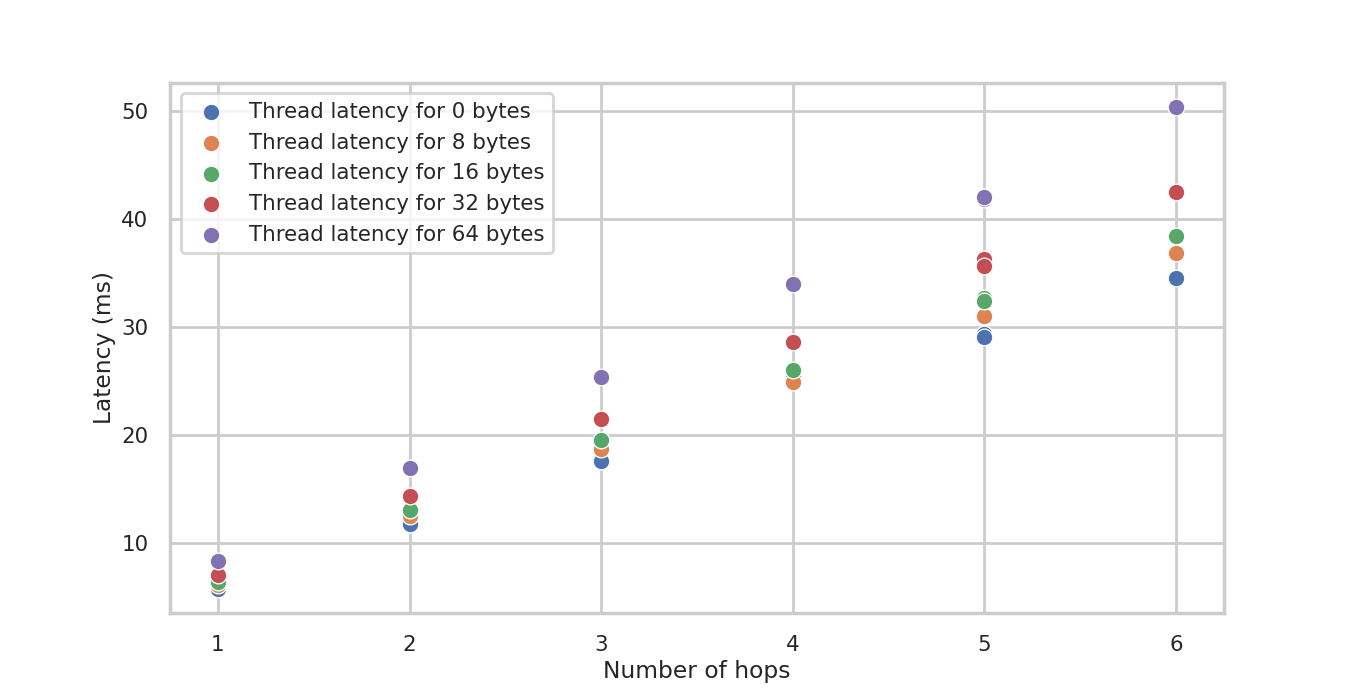
\includegraphics[scale=0.45]{images/Thread_Latency_all.png}
    \caption{Latency in Thread network dependent on the number of hops.}
    \label{fig:thread_latency_all}
\end{figure}

\begin{figure}[H]
    \centering
    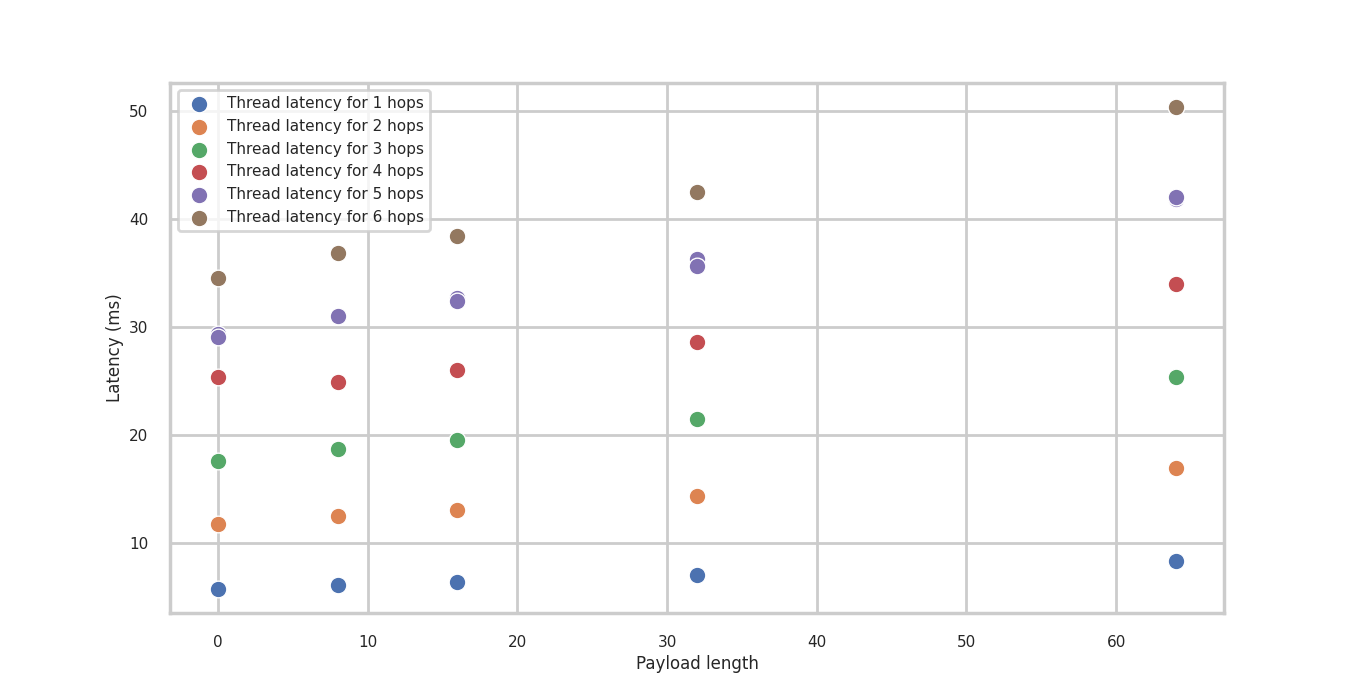
\includegraphics[scale=0.45]{images/Thread_Latency_vs_length.png}
    \caption{Latency in Thread network dependent on the payload length. }
    \label{fig:thread_latency_length}
\end{figure}

\subsection{Latency in Zigbee networks}

\begin{figure}[H]
    \centering
    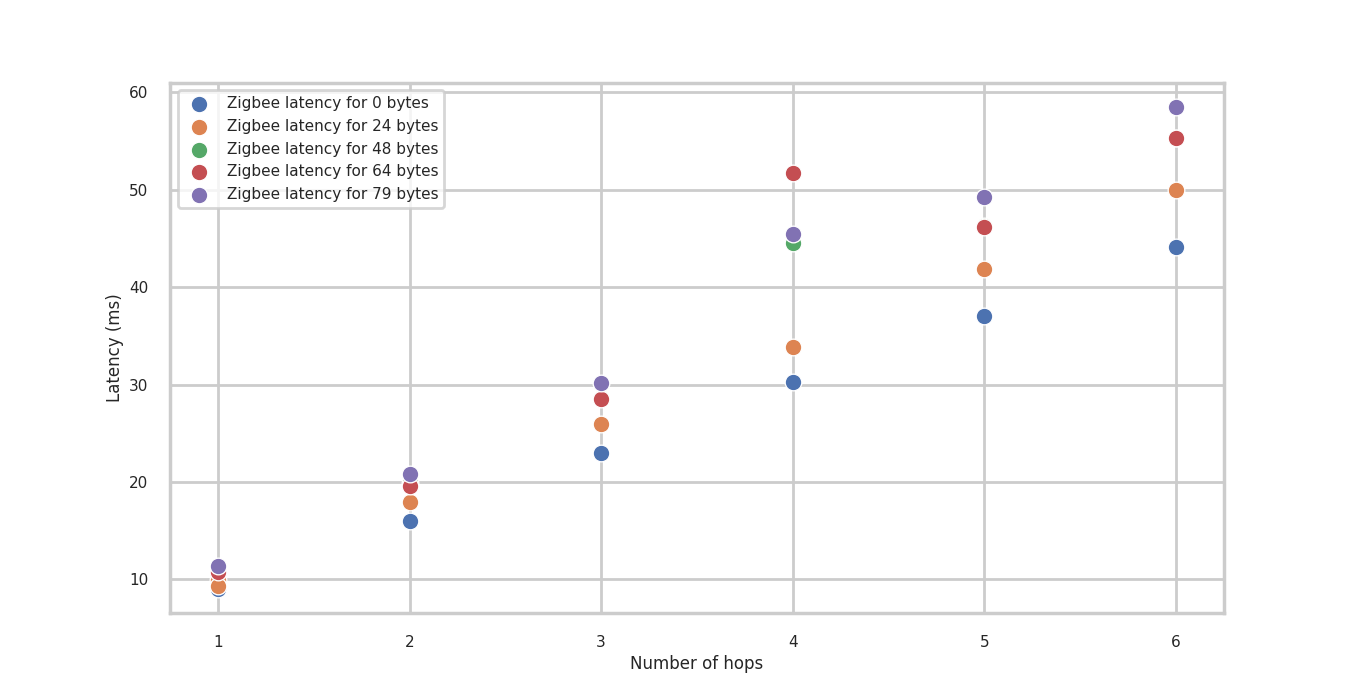
\includegraphics[scale=0.45]{images/Zigbee_Latency_all.png}
    \caption{Latency in Zigbee network dependent on the number of hops.}
    \label{fig:zigbee_latency_all}
\end{figure}

\begin{figure}[H]
    \centering
    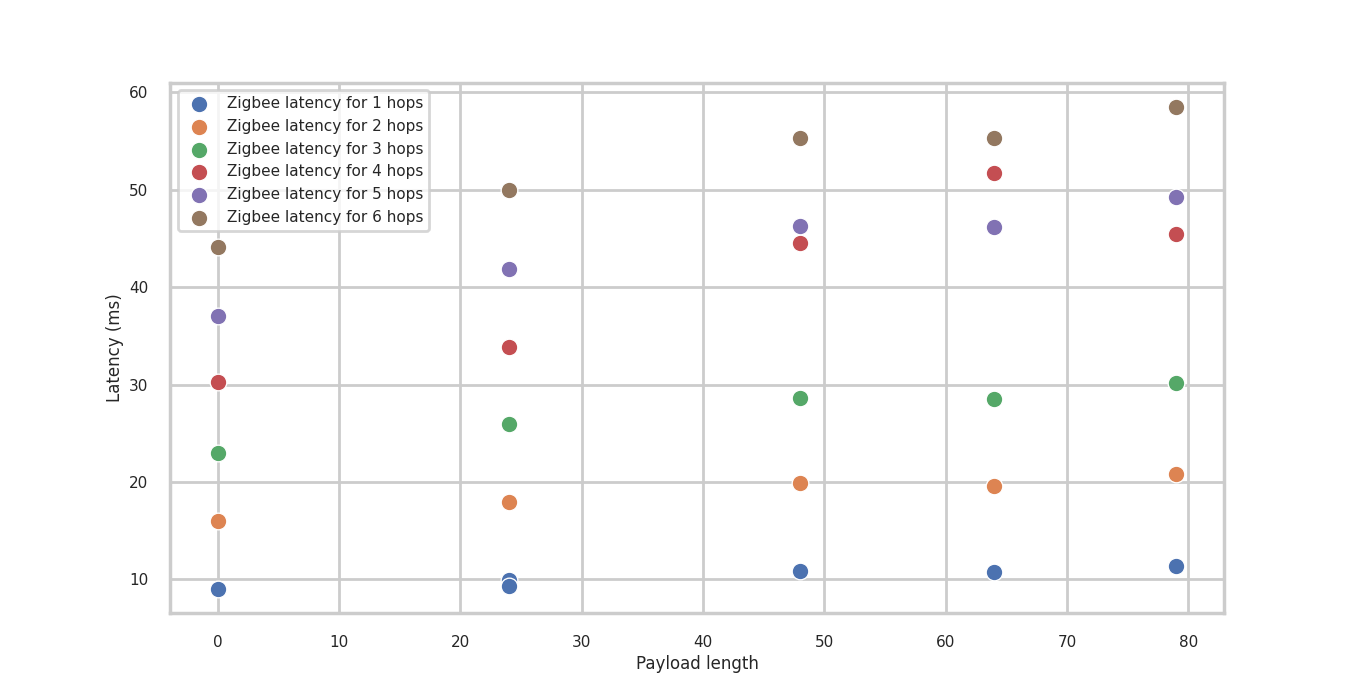
\includegraphics[scale=0.45]{images/Zigbee_Latency_vs_length.png}
    \caption{Latency in Zigbee network dependent on the payload length. }
    \label{fig:zigbee_latency_length}
\end{figure}

\section{Throughput}
\subsection{Throughput in Thread networks}

\begin{figure}[H]
    \centering
    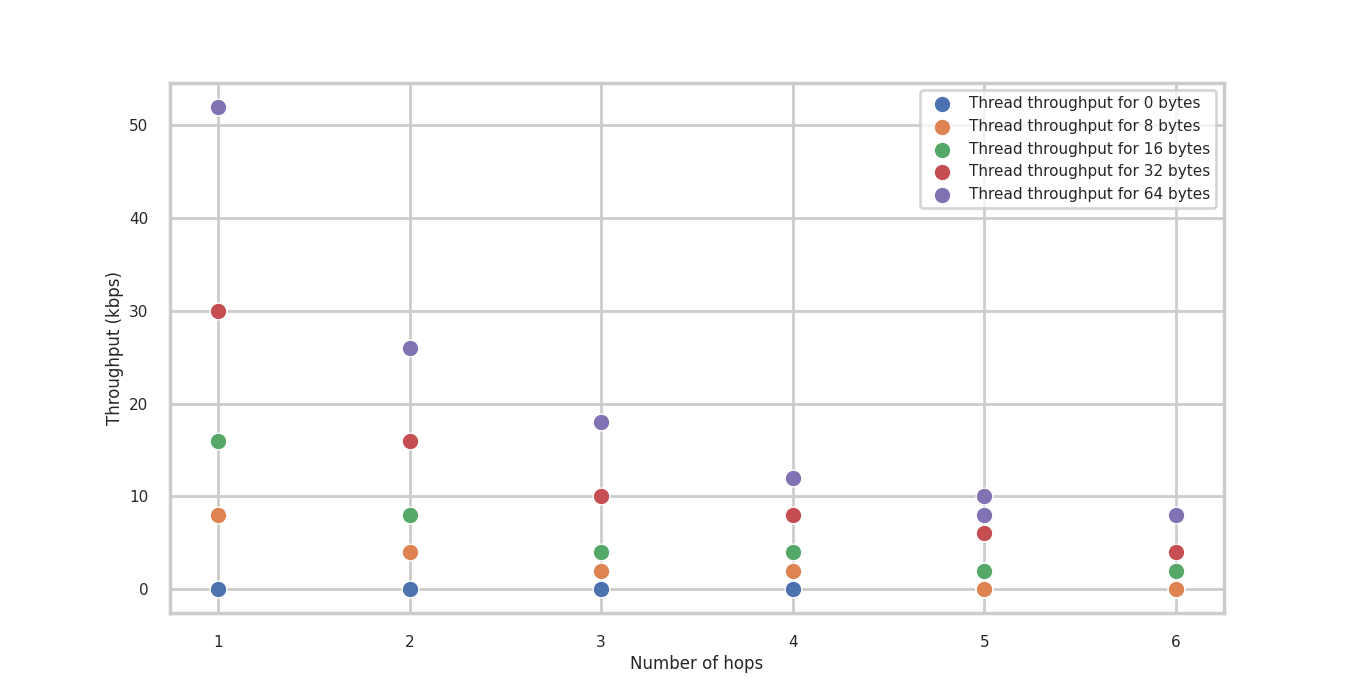
\includegraphics[scale=0.45]{images/Thread_Throughput_all.png}
    \caption{Throughput in Thread network dependent on the number of hops.}
    \label{fig:thread_throughput_all}
\end{figure}

\begin{figure}[H]
    \centering
    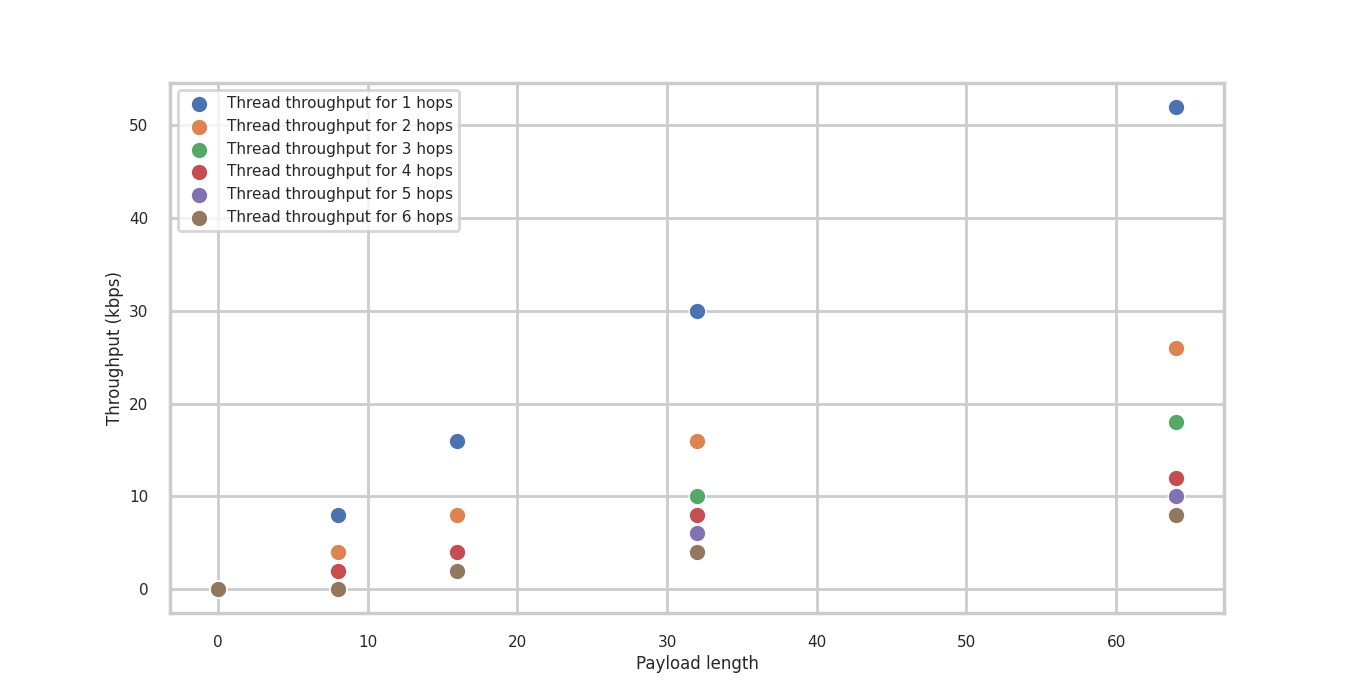
\includegraphics[scale=0.45]{images/Thread_Throughput_vs_length.png}
    \caption{Throughput in Thread network dependent on the payload length. }
    \label{fig:thread_throughput_length}
\end{figure}


\subsection{Throughput in Zigbee networks}

\begin{figure}[H]
    \centering
    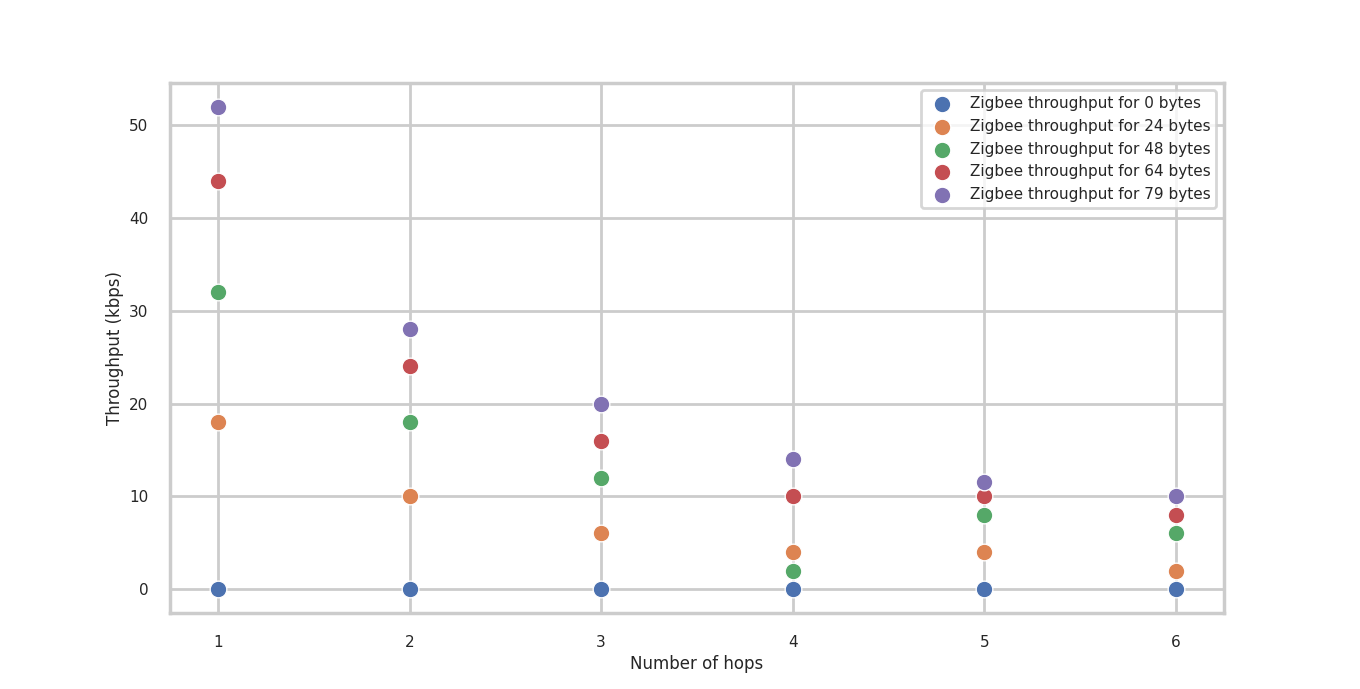
\includegraphics[scale=0.45]{images/Zigbee_Throughput_all.png}
    \caption{Throughput in Zigbee network dependent on the number of hops.}
    \label{fig:zigbee_throughput_all}
\end{figure}

\begin{figure}[H]
    \centering
    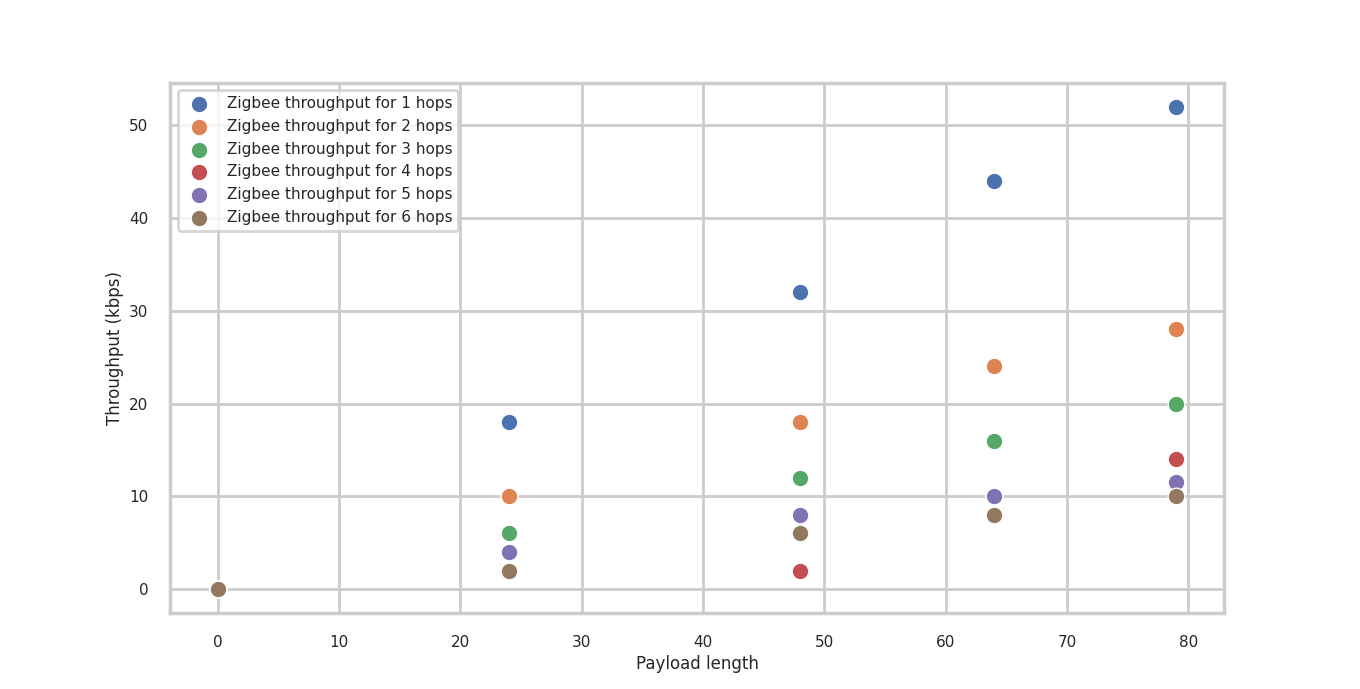
\includegraphics[scale=0.45]{images/Zigbee_Throughput_vs_length.png}
    \caption{Throughput in Zigbee network dependent on the payload length. }
    \label{fig:zigbee_throughput_length}
\end{figure}

\section{Performance comparison}

\begin{figure}[H]
    \centering
    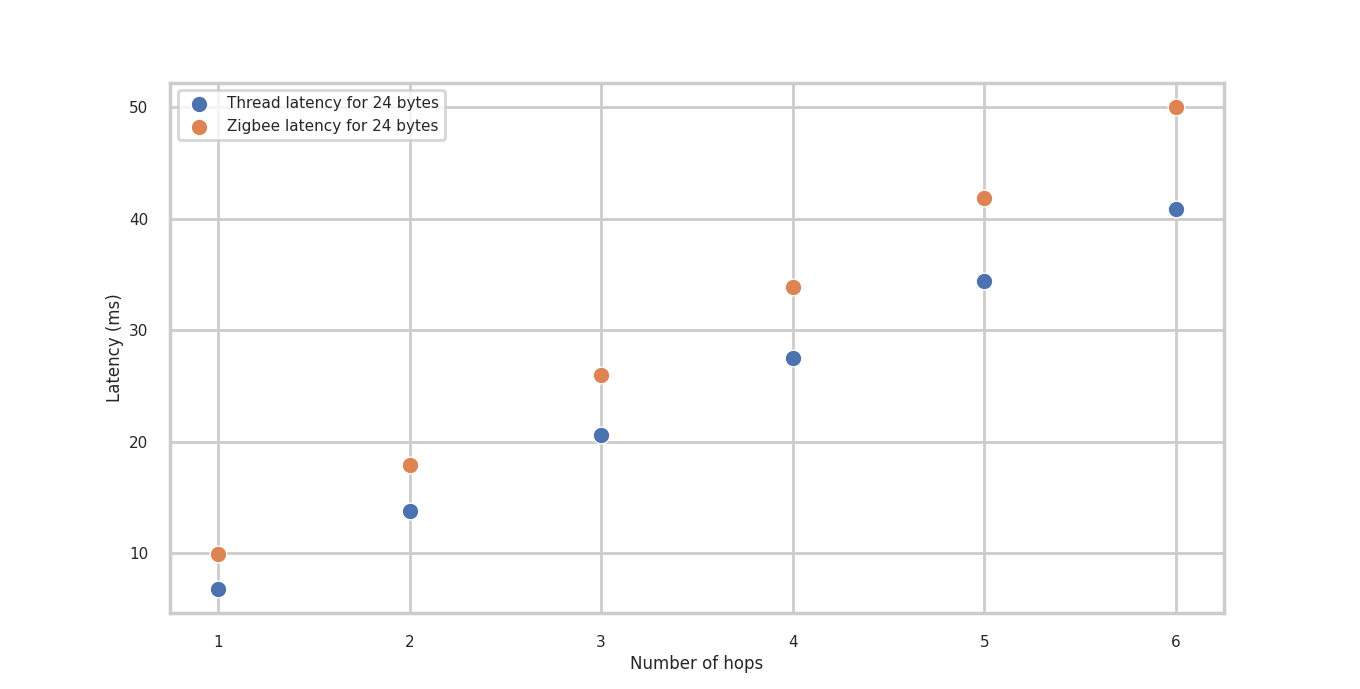
\includegraphics[scale=0.45]{images/Thread_vs_Zigbee_Latency.png}
    \caption{TODO.}
    \label{fig:thread_vs_zigbee_latency}
\end{figure}

\begin{figure}[H]
    \centering
    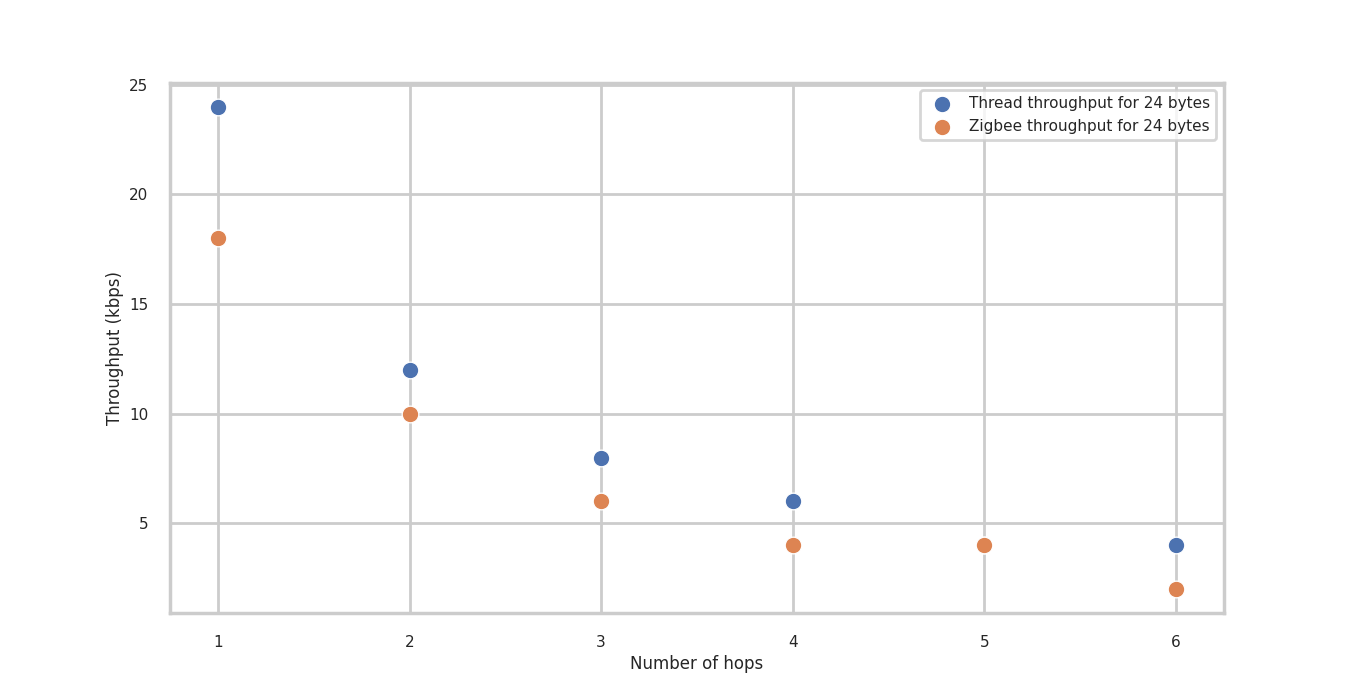
\includegraphics[scale=0.45]{images/Thread_vs_Zigbee_Throoughput.png}
    \caption{TODO.}
    \label{fig:thread_vs_zigbee_throughput}
\end{figure}
